% !TEX program  = pdflatex
% CVPR 2022 Paper Template
% based on the CVPR template provided by Ming-Ming Cheng (https://github.com/MCG-NKU/CVPR_Template)
% modified and extended by Stefan Roth (stefan.roth@NOSPAMtu-darmstadt.de)

\documentclass[10pt,twocolumn,letterpaper]{article}

%%%%%%%%% PAPER TYPE  - PLEASE UPDATE FOR FINAL VERSION
\usepackage[final]{cvpr}      % To produce the REVIEW version
%\usepackage{cvpr}              % To produce the CAMERA-READY version
%\usepackage[pagenumbers]{cvpr} % To force page numbers, e.g. for an arXiv version

% Include other packages here, before hyperref.
\usepackage{graphicx}
\usepackage{amsmath}
\usepackage{amssymb}
\usepackage{bm}
\usepackage{booktabs}


% It is strongly recommended to use hyperref, especially for the review version.
% hyperref with option pagebackref eases the reviewers' job.
% Please disable hyperref *only* if you encounter grave issues, e.g. with the
% file validation for the camera-ready version.
%
% If you comment hyperref and then uncomment it, you should delete
% ReviewTempalte.aux before re-running LaTeX.
% (Or just hit 'q' on the first LaTeX run, let it finish, and you
%  should be clear).
\usepackage[pagebackref,breaklinks,colorlinks]{hyperref}


% Support for easy cross-referencing
\usepackage[capitalize]{cleveref}
\crefname{section}{Sec.}{Secs.}
\Crefname{section}{Section}{Sections}
\Crefname{table}{Table}{Tables}
\crefname{table}{Tab.}{Tabs.}


% \usepackage{mathrsfs}





\usepackage{algorithm}
\usepackage{algorithmicx}
\usepackage{algpseudocode} 
\renewcommand{\algorithmicrequire}{ \textbf{Input:}}       
\renewcommand{\algorithmicensure}{ \textbf{Output:}} 



%%%% Commands
\usepackage{ifthen}
\usepackage{xifthen}
\def\*#1{\mathbf{#1}} \def\+#1{\mathcal{#1}} \def\-#1{\mathrm{#1}}\def\^#1{\mathbb{#1}}\def\!#1{\mathtt{#1}}
% \def\@#1{\mathscr{#1}}
\newcommand{\set}[1]{\left\{#1\right\}}
\newcommand{\tuple}[1]{\left(#1\right)} \newcommand{\eps}{\varepsilon}
\newcommand{\inner}[2]{\langle #1,#2\rangle} \newcommand{\tp}{\tuple}
\renewcommand{\mid}{\;\middle\vert\;} \newcommand{\cmid}{\,:\,}
\newcommand{\numP}{\#\mathbf{P}} \renewcommand{\P}{\mathbf{P}}
\newcommand{\defeq}{\triangleq} \renewcommand{\d}{\,\-d}
\newcommand{\ol}{\overline}
\newcommand{\argmin}{\mathop{\arg\min}}
\renewcommand{\Pr}[2][]{ \ifthenelse{\isempty{#1}}
  {\mathbf{Pr}\left[#2\right]} {\mathbf{Pr}_{#1}\left[#2\right]} }
\newcommand{\E}[2][]{ \ifthenelse{\isempty{#1}}
  {\mathbb{E}\left[#2\right]}
  {\mathbb{E}_{#1}\left[#2\right]} }
\newcommand{\Var}[2][]{ \ifthenelse{\isempty{#1}}
  {\mathbf{Var}\left[#2\right]}
  {\mathbf{Var}_{#1}\left[#2\right]} }
\newcommand{\Ent}[2][]{ \ifthenelse{\isempty{#1}}
  {\mathbf{Ent}\left[#2\right]}
  {\mathbf{Ent}_{#1}\left[#2\right]} }
\renewcommand{\emptyset}{\varnothing}
\providecommand{\lxor}{\oplus}
\newcommand{\start}[1]{\mathrm{start}\left(#1\right)}
\newcommand{\finish}[1]{\mathrm{finish}\left(#1\right)}
\newcommand{\depth}[1]{\mathrm{depth}\left(#1\right)}
\newcommand{\lis}[1]{\mathrm{LIS}\left(#1\right)}
\newcommand{\marked}[1]{\mathrm{marked}\left[#1\right]}
\newcommand{\tdist}[1]{\mathrm{tdist}\left[#1\right]}
\newcommand{\dist}[2][]{ \ifthenelse{\isempty{#1}}
  {\mathrm{dist}\left[#2\right]}
  {\mathrm{dist}_{#1}\left[#2\right]} }
\newcommand{\pre}[1]{\mathrm{pre}\left[#1\right]}
\newcommand{\cost}[1]{\mathrm{cost}\left[#1\right]}
\newcommand{\rank}[1]{\mathrm{rank}\left[#1\right]}
\newcommand{\ed}[1]{\mathrm{ED}\left[#1\right]}
\newcommand{\hinge}[1]{\mathrm{Hinge}\left[#1\right]}
\newcommand{\true}{\texttt{true}}
\newcommand{\false}{\texttt{false}}
\newcommand{\p}{\textbf{P}}
\newcommand{\np}{\textbf{NP}}
\newcommand{\opt}{\mathrm{OPT}}
\newcommand{\reduce}{\leq_k}


\newcommand{\norm}[2][]{ \ifthenelse{\isempty{#1}}
  {\left\|#2\right\|}
  {\left\|#2\right\|_{#1}} }
%%%%

\begin{document}

%%%%%%%%% TITLE - PLEASE UPDATE
\title{NLP project: Frameworks for Chinese Spoken Language Understanding}

\author{Yuchen Hou*, Xianhan Yu*, Siyu Pan*\\
Shanghai Jiaotong University, Shanghai, China}


\maketitle

\renewcommand{\thefootnote}{\fnsymbol{footnote}}
\footnotetext[1]{Equal contribution.}
\renewcommand{\thefootnote}{\arabic{footnote}}

\section{Abstract}
Spoken language understanding (SLU) is an emerging field in between the areas of speech processing
and natural language processing. It is an critical part of conversation system, which aims to extract
users’ intention and s the foundation for follow-ups.In this work, we mainly focus on how to improve the effect of information extraction, we not only sophisticatedly train the given baseline model, but also try many recently widely-concerned models in SLU, such as Bi-LSTM-CRF, Bert-CRF and  Transformer-CRF. The accuracy of the baseline model on given dataset reaches 71.06$\%$, and the accuracy of our best model Transformer-CRF reaches 87.49$\%$.

\section{Problem Definition}
Fig. 1(a) shows a diagram of Spoken dialogue system, which includes five parts. Our task focuses on
the SLU part, which takes words as input and outputs their semantics. Specifically, the task can be seen as a multi-class classification, which assigns BIO labels to input. The BIO annotation labels each word as B-X, I-X, or O, where X is the category of a fragment. In general, B-X means this word is at the beginning of a fragment, and the fragment belongs to category X,I-X means this word is at the end of a fragment and the fragment belongs to category X, and O means this word doesn't belong to any valid fragment, which indicates no semantic information.
\begin{figure}[htbp]
	\centering
	\begin{minipage}{0.48\linewidth}
		\centering
		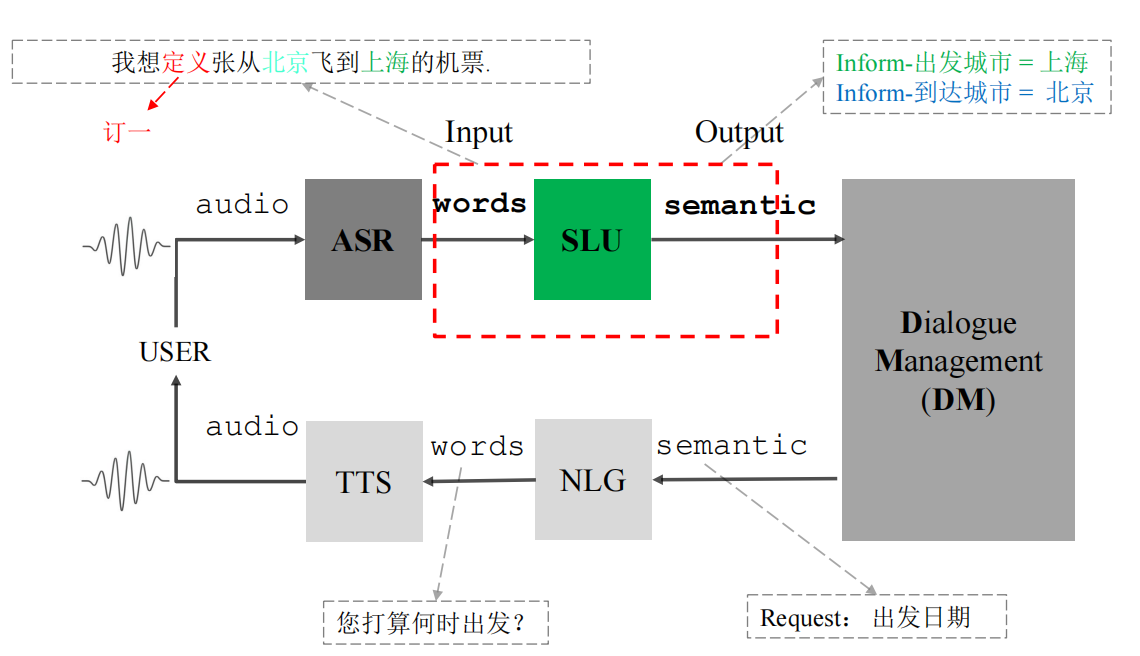
\includegraphics[height=3cm,width=4cm]{graph/g1.png}
		\label{fig1}
	\end{minipage}
	\begin{minipage}{0.48\linewidth}
		\centering
		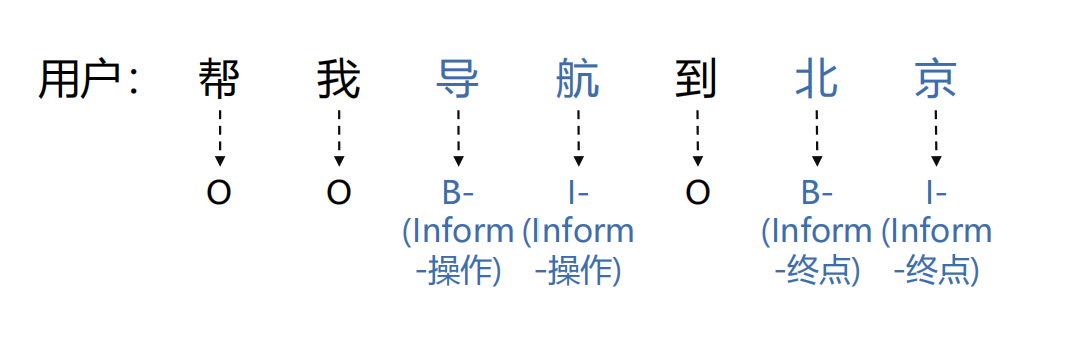
\includegraphics[height=1.5cm,width=4cm]{graph/g2.png}
		\label{fig2}
	\end{minipage}
	\caption{(a) A diagram of Spoken dialogue system. (b) An example of BIO annotation. In (b), Act-slot can be combined as a tag and then we can use the B-[Act plot] and I-[Act plot] tags to determine the value.}
\end{figure}
\section{Method}
\subsection{Base Processing}
In problem definition section, we introduce the BIO annotation:B-X,I-X and O, where X means the type of fragment.In our dataset, there are 2 types of action and 18 types of slots. We add a type of [PAD] to represent the padding word, so there are  totally 74 (36$\times$2+1+1) tags in our dataset.We then convert the SLU problem into a multi-class classification task. 

In our model, all of the words in the input sequences are denoted by indexes and embedded as vectors by pretrained word embedding. Since
the length of input sequence in a batch should be uniform, we pad the sequence to the max length of the input sequence in a batch and construct a mask to distinguish the original sequence and the padding part. 

\subsection{Models}
\subsubsection{Bi-RNN}
In baseline model, bidirecrional RNN acts as the encoder. For each word in the input sequence, each layer computes the following function:
\begin{equation}
    h_t = tanh(w_{ih}x_t + b_{ih} + w_{hh}h_{t−1} + b_{hh})
\end{equation}
where h\_t is the hidden state at time t, x\_t is the input at time t, and h\_{t-1} is the hidden state of the previous layer at time t − 1 or the initial hidden state at time o.

\begin{figure}[htbp]
	\centering
	\begin{minipage}{0.45\linewidth}
		\centering
		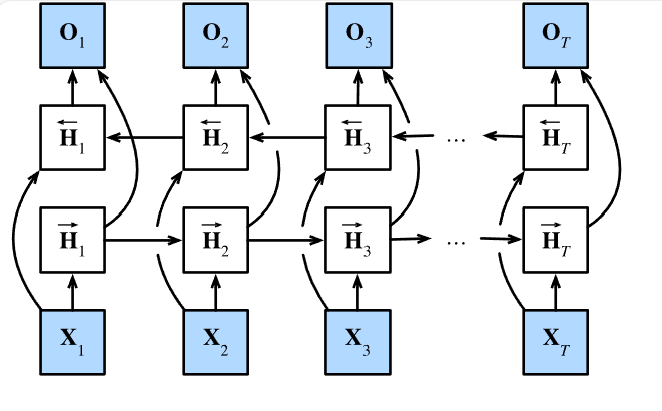
\includegraphics[height=3cm,width=3.7cm]{graph/fig5.png}
		\label{fig5}
	\end{minipage}
	\begin{minipage}{0.53\linewidth}
		\centering
		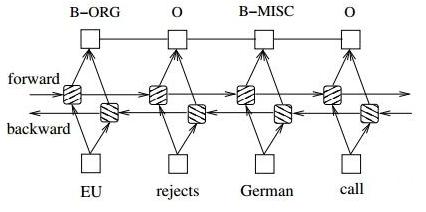
\includegraphics[height=3cm,width=4.3cm]{graph/fig6.jpg}
		\label{fig6}
	\end{minipage}
	\caption{(a)Architecture of Bi-RNN. (b)Architecture of Bi-LSTM }
\end{figure}

\subsubsection{Bi-LSTM}
In baseline model, we replace bi-RNN with bidirectional long short term memory (LSTM) as the encoder. For each word in the input sequence, each layer computes the following function:
\begin{equation}
    \begin{split}
    & i_t = sigmoid(W_{ii}x_t + b_{ii} + W_{hi}h_{t-1} + b_{hi}) \\
    & f_t = sigmoid(W_{if}x_t + b_{if} + W_{hf}h_{t-1} + b_{hf}) \\
    & o_t = sigmoid(W_{io}x_t + b_{io} + W_{ho}h_{t-1} + b_{ho}) \\
    & g_t = tanh(W_{ig}x_t + b_{ig} + W_{hg}h_{t-1} + b_{hg})\\
    & c_t = f_tc_{t-1} + i_tg_t \\
    & h_t = o_t * tanh(c_t)
    \end{split}
\end{equation}
where h\_t is the hidden state at time t, c\_t is the cell state at time t, x\_t is the input at time t, h\_{t−1} is the hidden state of the layer at time t − 1 or the initial hidden state at time o. i\_t, f\_t, g\_t, ot are the input, forget, cell, and output gates, respectively.

\subsubsection{Bi-LSTM-CRF}

Conditional random field considers the correlation between labels, thus adding some constraints to prevent undesirable conditions, such as I-Y after B-X. We add the CRF layer after Bi-LSTM layer to improve model's performance.

\begin{figure}[htb]
  \centering
  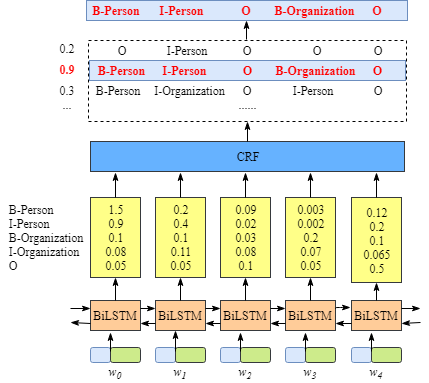
\includegraphics[height=8cm,width=8cm]{graph/fig3.png}
  \caption{Architecture of Bi-LSTM-CRF}
  \label{fig3}
\end{figure}

\subsubsection{BERT-CRF}

Bidirectional Encoder Representation from Transformers(BERT) is one of the most successful models in NLP in recent years, and there are many pretrained models for BERT.

We use BERT to replace the Bi-LSTM layer in Bi-LSTM-CRF. The pretrained model we choose is chinese-bert-wwm-ext, which is pretrained on Chinese Wikipedia and other general data including Q\&A conversations and news. Besides, in word to vector step, we also used the word embedding from BERT.

\subsubsection{Transformer-CRF}

The Transformer model~\cite{transformer} has emerged as another landmark in the field of NLP in recent years. In our variant of this model, the encoder component is substituted with a streamlined Transformer architecture. We feed the embedded \texttt{input\_id} and \texttt{tag\_id} directly into the Transformer.
\begin{figure}[htbp]
    \centering
    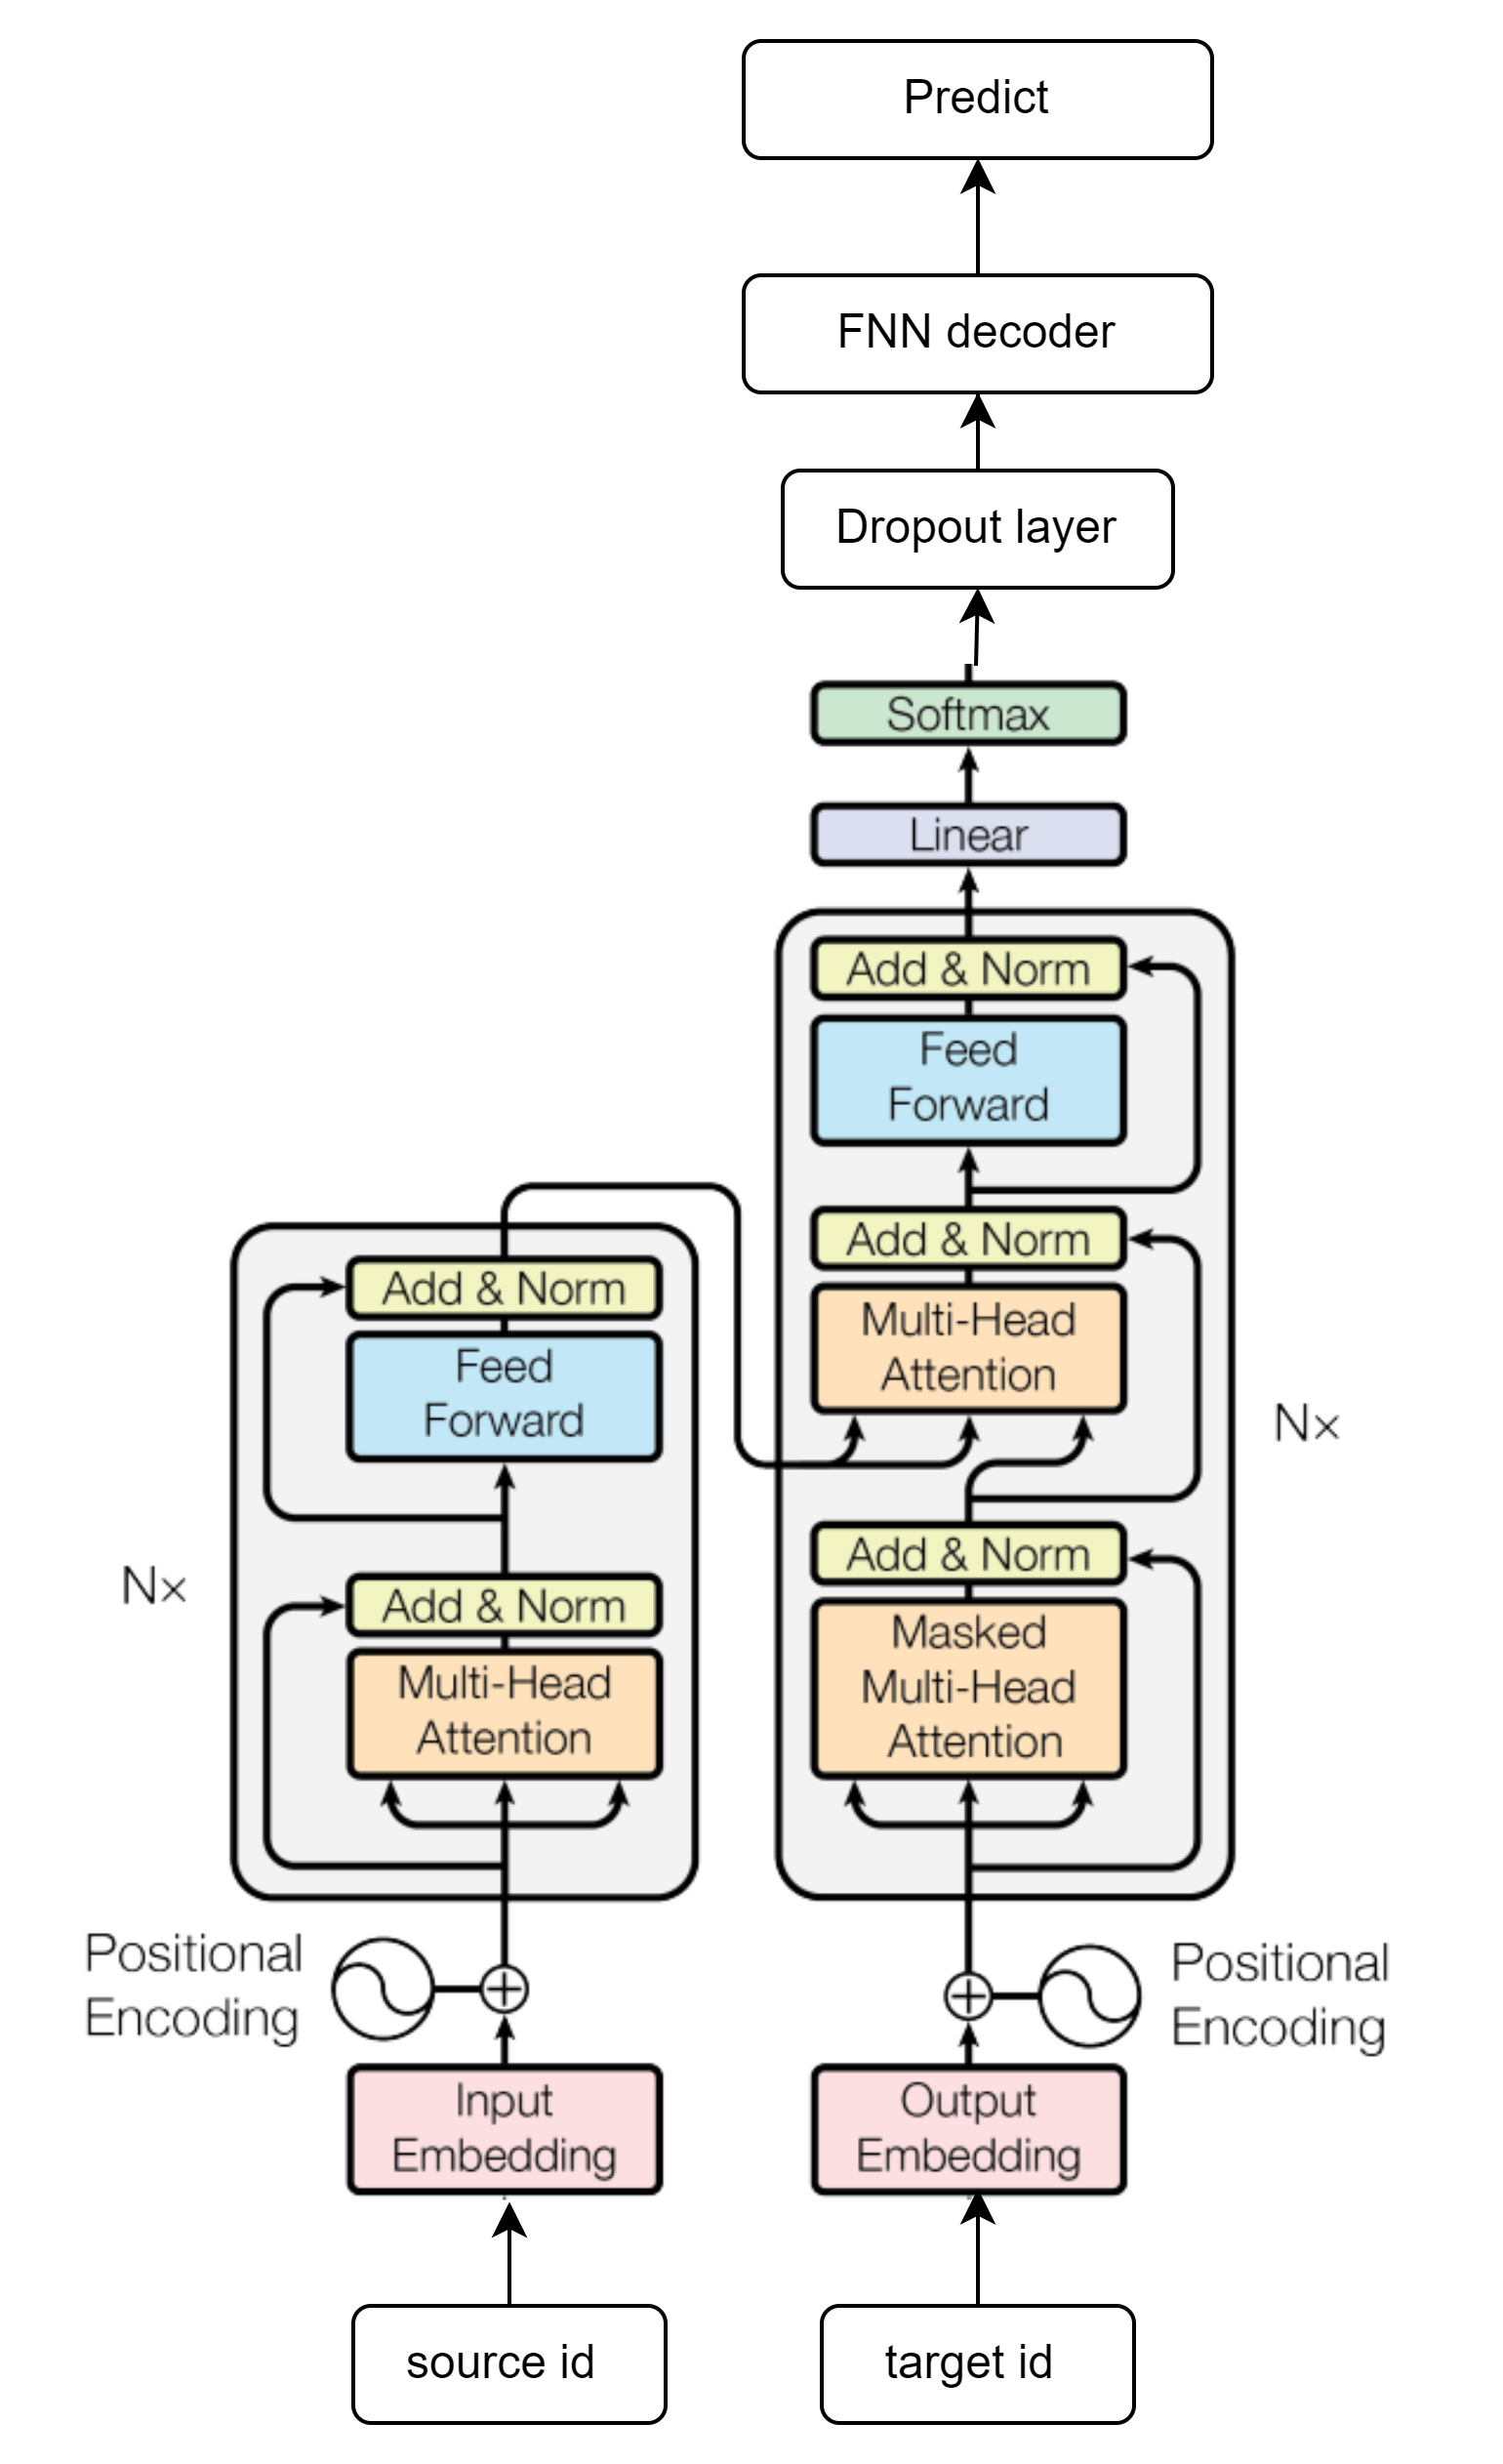
\includegraphics[width=0.9\linewidth]{graph/transformer.png}
    \caption{Transforer Stucture in SLUTagging}
    \label{fig:my_label}
\end{figure}
To preclude the possibility of future tokens influencing the prediction of current ones, we employ the \texttt{transformer.generate\_square\_subsequent\_mask} method. This ensures that, for any given position within the sequence, only the preceding elements are utilized during prediction.

The remainder of our baseline model persists without alteration. Furthermore, in the decoding phase—translating model outputs into labels—we optionally incorporate a CRF (Conditional Random Fields) layer to refine our evaluations.


\subsection{Anti Noise}
We define a function \texttt{anti\_noise\_prediction} to refine the predictions based on the decoder's output. This function's primary role is to correct the results of the SLU system to align with the predefined vocabulary specified in \texttt{ontology.json}.

 It checks these predictions with a set of predefined location names (e.g. 'poi name', 'start name'. If the label in the prediction is not 'value' but one of the above positions or categories, it tries to correct it by finding the closest valid slot (slot) value.

The \texttt{LabelVocab} class retrieves the pinyin set \texttt{pinyin\_set} of all POI names from the file \texttt{/data/lexicon/poi\_name.txt} along with the mapping dictionary \texttt{map\_dic}. It checks if the noise is directly in \texttt{pinyin\_set}, and if so, returns the corresponding value directly. 

If not, it calculates the Jaccard similarity between the noise and each element in \texttt{pinyin\_set}, selecting the one with the highest similarity.

\[
J(A, B) = \frac{|A \cap B|}{|A \cup B|}
\]

This method is a heuristic search that assumes that pinyin pairs with more shared elements are more similar. 

\section{Experiments}
\subsection{Model Comparison}
\begin{table}[htbp]
\centering
\resizebox{0.45\textwidth}{!}{
\begin{tabular}{c c c c c}
    \toprule[0.4mm]
    \textbf{Model} & \textbf{Accuracy} & \textbf{Precision} &\textbf{Recall} & \textbf{F1 Score}  \\
    % \hline
    \midrule[0.25mm]
    Bi-RNN  &  70.83 & 79.91 & 73.93 & 76.75\\
    Bi-LSTM & 71.06 & 80.85 & 73.51 & 77.01\\
    GRU & 71.95 & 81.37 & 75.18 & 78.15\\
    \midrule[0.25mm]
    BERT & 76.31 & 82.51 & 80.02 & 81.25\\
    Transformer & \textbf{87.49} & \text{99.88} & \textbf{88.32} & \textbf{93.75}  \\
    % \hline
    \midrule[0.25mm]
    Bi-RNN-CRF  & 72.18 & 84.35 & 74.77 & 79.27\\
    Bi-LSTM-CRF & 73.28 & 85.29 & 76.11 & 79.53\\
    GRU-CRF & 73.88 & 86,32 & 76.12 & 79.89
    \midrule[0.25mm]
    BERT-CRF & 78.99 & 81.25 & 78.62 & 79.92\\
    % \hline
    Transformer-CRF  & \textbf{87.49} & \text{99.88} & \textbf{88.32} & \textbf{93.75}  \\
    % \hline
    \bottomrule[0.4mm]
\end{tabular}}
\caption{ the evaluation results of all the models}
\label{tab1}
\end{table}

\begin{itemize}
    \item Tab\ref{tab1} displays models' performance on the given dataset. Transformer and Transformer-CRF equally perform best on the given dataset. BERT and Transformer, both with CRF layer and without CRF layer, outperform RNN and LSTM greatly. Besides, the results show that models (except Transformer) with CRF layer outperform the corresponding models without CRF layer about 1\% in accuracy. Such improvements suggest that CRF layer is valid for better prediction performance for spoken language understanding tasks.
    
    The reason why CRF layer doesn't improve the Transformer's performance may be the given dataset is small, only Transformer can learn the constraints between labels. If we want to study whether Transformer has the ability to learn the constraints, we need larger and more complex dataset.
    \item The results also show that Baseline-GRU beats all the other baselines.GRU is an efficient encoder compared to LSTM RNN, so we use GRU in subsequent references to the transformer and BERT.
\end{itemize}


\begin{figure}[htbp]
	\centering
	\begin{minipage}{0.32\linewidth}
		\centering
		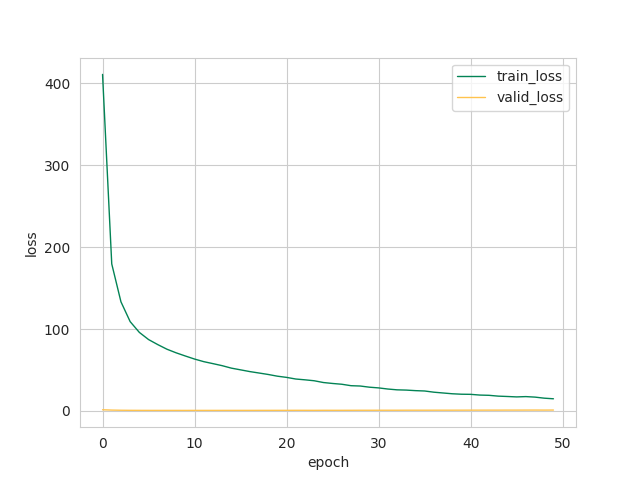
\includegraphics[height=2cm,width=2.7cm]{graph/rnn.png}
		\label{fig5}
	\end{minipage}
	\begin{minipage}{0.32\linewidth}
		\centering
		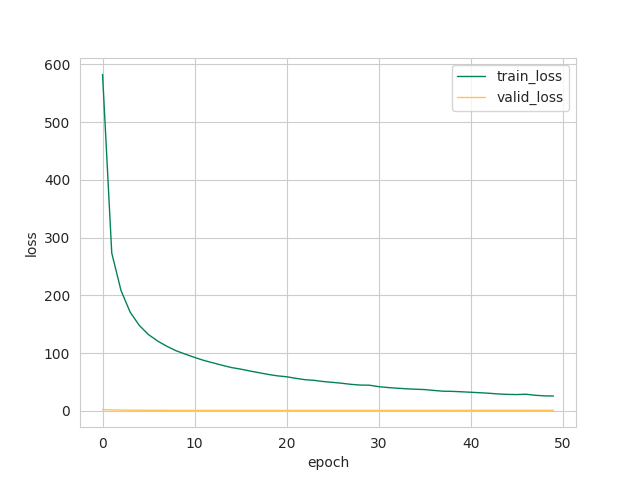
\includegraphics[height=2cm,width=2.7cm]{graph/lstm.png}
		\label{fig6}
	\end{minipage}
	\begin{minipage}{0.32\linewidth}
		\centering
		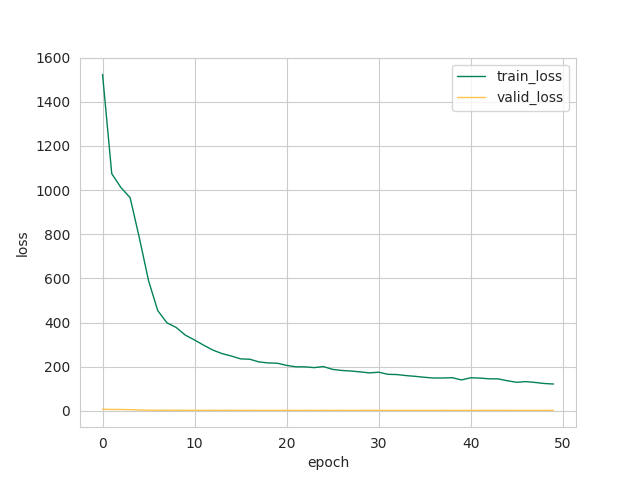
\includegraphics[height=2cm,width=2.7cm]{graph/bert-lstm.png}
		\label{fig6}
	\end{minipage}
	\caption{ The training and validation loss of the Bi-RNN-CRF, Bi-LSTM-CRF and BERT-CRF.}
\end{figure}

\subsection{Impact of Noise}
\begin{table}[htbp]
\centering
\resizebox{0.45\textwidth}{!}{
\begin{tabular}{c c c c c}
    \toprule[0.4mm]
    \textbf{Model} & \textbf{Accuracy} & \textbf{Precision} &\textbf{Recall} & \textbf{F1 Score}  \\
    % \hline
    \midrule[0.25mm]
    GRU & 71.95 & 81.37 & 75.18 & 78.15\\
    GRU_anti-noise & 72.13 & 81.02 & 77.23 & 78.32\\
    \midrule[0.25mm]
    Transformer & \textbf{87.49} & \text{99.88} & \textbf{88.32} & \textbf{93.75}  \\
    Transformer & \textbf{87.52} & \text{99.32} & \textbf{89.12} & \textbf{94.23}  \\
    % \hline
    \bottomrule[0.4mm]
\end{tabular}}
\end{table}

\section{Conclusion}
In this work, we mainly focus on how to improve the effect of information extraction, we not only sophisticatedly train the given baseline model, but also train BERT and Transformer on the given dataset. Besides, we add a CRF layer to learn the constraints between labels for better performance. The accuracy of the baseline model on given dataset reaches 71.06$\%$, and the accuracy of our best model Transformer-CRF reaches 87.49$\%$.


\section{Outlook}
\subsection{Pinyin-Based Noise Mitigation}

To counteract the noise stemming from misinterpretations in our anti-noise module, we employ the Jaccard Similarity Index to ascertain the value that most closely aligns in pinyin similarity. For more intricate applications, the adoption of sophisticated string or pinyin similarity algorithms might be warranted. These could include methods like the edit distance—specifically, the Levenshtein distance—or phonetic and rhyming schemes for a more nuanced matching.
\subsection{Data Augmentation}

To help the model generalize better to new and unseen data, especially if the training data is limited or skewed, we added data argumentation. Specifically, data argumentation methods include speech transformation (changing pitch, speed, or accent), text expansion (using synonym replacement, sentence reconstruction), noise injection (adding background noise), and data synthesis (generating entirely new speech or text data).

%%%%%%%%% REFERENCES
{\small
\bibliographystyle{ieee_fullname}
\bibliography{main}
}

 

\end{document}
